\documentclass{standalone}
\usepackage{tikz}
\usetikzlibrary{patterns, positioning}


\begin{document}
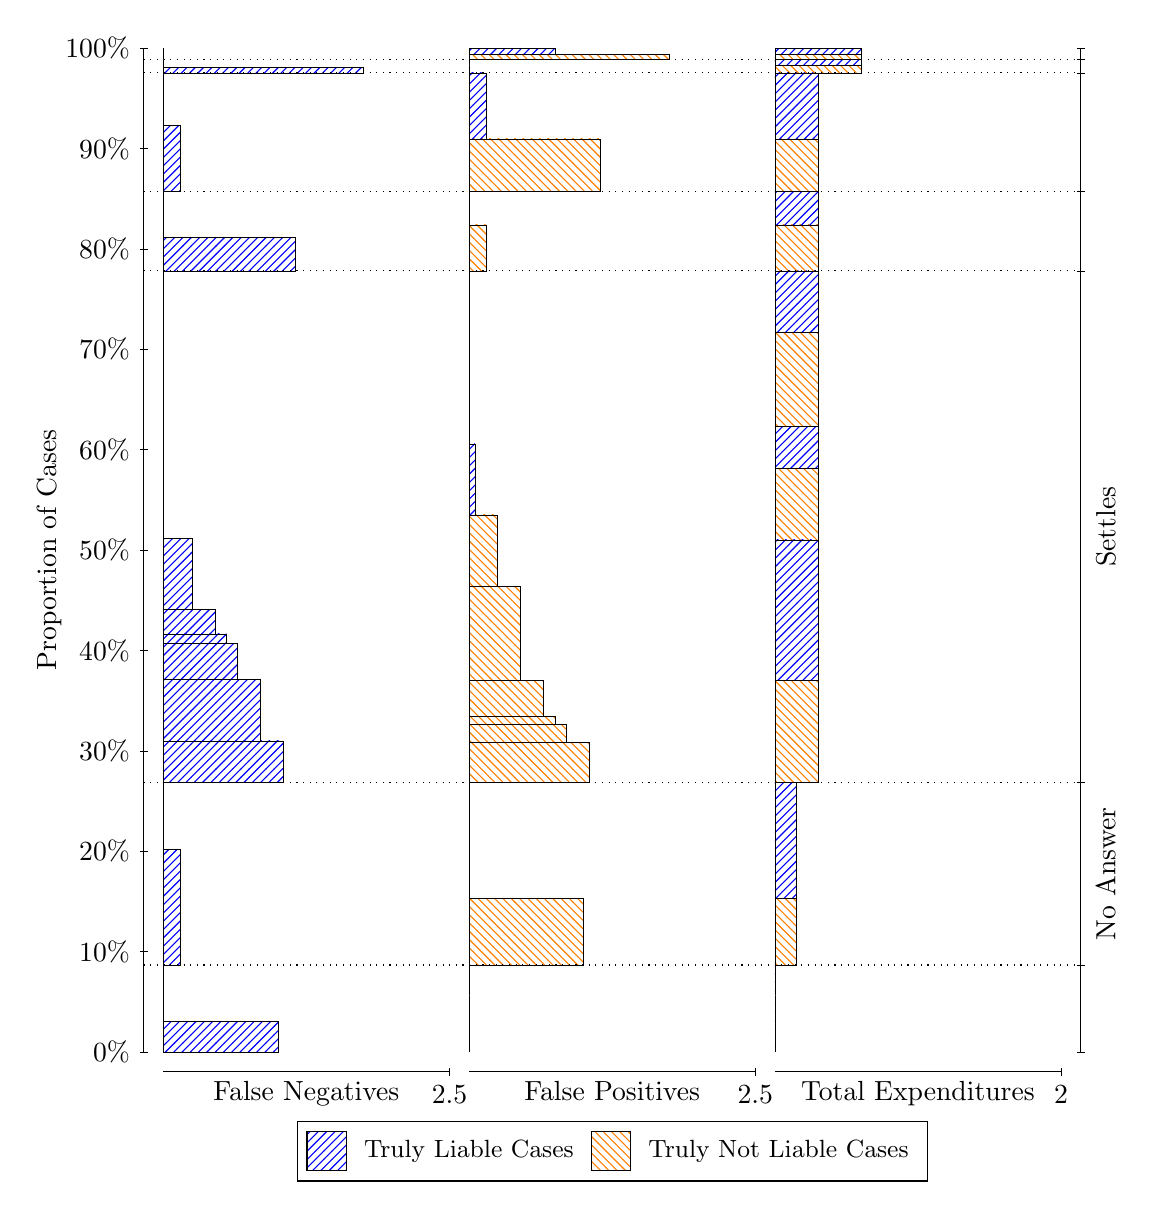
\begin{tikzpicture}
\draw[black, very thin] (1.5,1.75) -- (1.5,14.5);
\node[rotate=90, text=black, anchor=center] at (0.3, 8.125) {Proportion of Cases};
\draw[black, very thin] (1.45,1.75) -- (1.55,1.75);
\node[text=black, anchor=east] at (1.45, 1.75) {0\%};
\draw[black, very thin] (1.45,3.025) -- (1.55,3.025);
\node[text=black, anchor=east] at (1.45, 3.025) {10\%};
\draw[black, very thin] (1.45,4.3) -- (1.55,4.3);
\node[text=black, anchor=east] at (1.45, 4.3) {20\%};
\draw[black, very thin] (1.45,5.575) -- (1.55,5.575);
\node[text=black, anchor=east] at (1.45, 5.575) {30\%};
\draw[black, very thin] (1.45,6.85) -- (1.55,6.85);
\node[text=black, anchor=east] at (1.45, 6.85) {40\%};
\draw[black, very thin] (1.45,8.125) -- (1.55,8.125);
\node[text=black, anchor=east] at (1.45, 8.125) {50\%};
\draw[black, very thin] (1.45,9.4) -- (1.55,9.4);
\node[text=black, anchor=east] at (1.45, 9.4) {60\%};
\draw[black, very thin] (1.45,10.675) -- (1.55,10.675);
\node[text=black, anchor=east] at (1.45, 10.675) {70\%};
\draw[black, very thin] (1.45,11.95) -- (1.55,11.95);
\node[text=black, anchor=east] at (1.45, 11.95) {80\%};
\draw[black, very thin] (1.45,13.225) -- (1.55,13.225);
\node[text=black, anchor=east] at (1.45, 13.225) {90\%};
\draw[black, very thin] (1.45,14.5) -- (1.55,14.5);
\node[text=black, anchor=east] at (1.45, 14.5) {100\%};

\draw[black, very thin] (13.4,1.75) -- (13.4,14.5);
\draw[black, very thin] (13.35,1.75) -- (13.45,1.75);
\node[anchor=west] at (13.35, 1.75) {};
\draw[black, very thin] (13.35,2.8545) -- (13.45,2.8545);
\node[anchor=west] at (13.35, 2.8545) {};
\draw[black, very thin] (13.35,5.1713) -- (13.45,5.1713);
\node[anchor=west] at (13.35, 5.1713) {};
\draw[black, very thin] (13.35,11.671) -- (13.45,11.671);
\node[anchor=west] at (13.35, 11.671) {};
\draw[black, very thin] (13.35,12.68) -- (13.45,12.68);
\node[anchor=west] at (13.35, 12.68) {};
\draw[black, very thin] (13.35,14.184) -- (13.45,14.184);
\node[anchor=west] at (13.35, 14.184) {};
\draw[black, very thin] (13.35,14.354) -- (13.45,14.354);
\node[anchor=west] at (13.35, 14.354) {};
\draw[black, very thin] (13.35,14.5) -- (13.45,14.5);
\node[anchor=west] at (13.35, 14.5) {};

\draw[black, very thin, pattern color=blue, pattern=north east lines] (1.75,1.75) rectangle (3.2033,2.1392);
\draw[black, very thin, pattern color=orange, pattern=north west lines] (1.75,2.1392) rectangle (1.75,2.8545);
\draw[black, very thin, pattern color=blue, pattern=north east lines] (1.75,2.8545) rectangle (1.968,4.3214);
\draw[black, very thin, pattern color=orange, pattern=north west lines] (1.75,4.3214) rectangle (1.75,5.1713);
\draw[black, very thin, pattern color=blue, pattern=north east lines] (1.75,5.1713) rectangle (3.276,5.7016);
\draw[black, very thin, pattern color=blue, pattern=north east lines] (1.75,5.7016) rectangle (2.9853,6.4862);
\draw[black, very thin, pattern color=blue, pattern=north east lines] (1.75,6.4862) rectangle (2.6947,6.9408);
\draw[black, very thin, pattern color=blue, pattern=north east lines] (1.75,6.9408) rectangle (2.5493,7.0587);
\draw[black, very thin, pattern color=blue, pattern=north east lines] (1.75,7.0587) rectangle (2.404,7.3704);
\draw[black, very thin, pattern color=blue, pattern=north east lines] (1.75,7.3704) rectangle (2.1133,8.2718);
\draw[black, very thin, pattern color=orange, pattern=north west lines] (1.75,8.2718) rectangle (1.75,11.671);
\draw[black, very thin, pattern color=blue, pattern=north east lines] (1.75,11.671) rectangle (3.4213,12.096);
\draw[black, very thin, pattern color=orange, pattern=north west lines] (1.75,12.096) rectangle (1.75,12.68);
\draw[black, very thin, pattern color=blue, pattern=north east lines] (1.75,12.68) rectangle (1.968,13.519);
\draw[black, very thin, pattern color=orange, pattern=north west lines] (1.75,13.519) rectangle (1.75,14.184);
\draw[black, very thin, pattern color=blue, pattern=north east lines] (1.75,14.184) rectangle (4.2933,14.259);
\draw[black, very thin, pattern color=orange, pattern=north west lines] (1.75,14.259) rectangle (1.75,14.354);
\draw[black, very thin, pattern color=orange, pattern=north west lines] (1.75,14.354) rectangle (1.75,14.421);
\draw[black, very thin, pattern color=blue, pattern=north east lines] (1.75,14.421) rectangle (1.75,14.5);
\draw[black, very thin, pattern color=orange, pattern=north west lines] (5.6333,1.75) rectangle (5.6333,2.4652);
\draw[black, very thin, pattern color=blue, pattern=north east lines] (5.6333,2.4652) rectangle (5.6333,2.8545);
\draw[black, very thin, pattern color=orange, pattern=north west lines] (5.6333,2.8545) rectangle (7.0867,3.7044);
\draw[black, very thin, pattern color=blue, pattern=north east lines] (5.6333,3.7044) rectangle (5.6333,5.1713);
\draw[black, very thin, pattern color=orange, pattern=north west lines] (5.6333,5.1713) rectangle (7.1593,5.6864);
\draw[black, very thin, pattern color=orange, pattern=north west lines] (5.6333,5.6864) rectangle (6.8687,5.9076);
\draw[black, very thin, pattern color=orange, pattern=north west lines] (5.6333,5.9076) rectangle (6.7233,6.0145);
\draw[black, very thin, pattern color=orange, pattern=north west lines] (5.6333,6.0145) rectangle (6.578,6.4691);
\draw[black, very thin, pattern color=orange, pattern=north west lines] (5.6333,6.4691) rectangle (6.2873,7.6611);
\draw[black, very thin, pattern color=orange, pattern=north west lines] (5.6333,7.6611) rectangle (5.9967,8.5703);
\draw[black, very thin, pattern color=blue, pattern=north east lines] (5.6333,8.5703) rectangle (5.706,9.4717);
\draw[black, very thin, pattern color=blue, pattern=north east lines] (5.6333,9.4717) rectangle (5.6333,11.671);
\draw[black, very thin, pattern color=orange, pattern=north west lines] (5.6333,11.671) rectangle (5.8513,12.255);
\draw[black, very thin, pattern color=blue, pattern=north east lines] (5.6333,12.255) rectangle (5.6333,12.68);
\draw[black, very thin, pattern color=orange, pattern=north west lines] (5.6333,12.68) rectangle (7.3047,13.345);
\draw[black, very thin, pattern color=blue, pattern=north east lines] (5.6333,13.345) rectangle (5.8513,14.184);
\draw[black, very thin, pattern color=orange, pattern=north west lines] (5.6333,14.184) rectangle (5.6333,14.279);
\draw[black, very thin, pattern color=blue, pattern=north east lines] (5.6333,14.279) rectangle (5.6333,14.354);
\draw[black, very thin, pattern color=orange, pattern=north west lines] (5.6333,14.354) rectangle (8.1767,14.421);
\draw[black, very thin, pattern color=blue, pattern=north east lines] (5.6333,14.421) rectangle (6.7233,14.5);
\draw[black, very thin, pattern color=orange, pattern=north west lines] (9.5167,1.75) rectangle (9.5167,2.4652);
\draw[black, very thin, pattern color=blue, pattern=north east lines] (9.5167,2.4652) rectangle (9.5167,2.8545);
\draw[black, very thin, pattern color=orange, pattern=north west lines] (9.5167,2.8545) rectangle (9.7892,3.7044);
\draw[black, very thin, pattern color=blue, pattern=north east lines] (9.5167,3.7044) rectangle (9.7892,5.1713);
\draw[black, very thin, pattern color=orange, pattern=north west lines] (9.5167,5.1713) rectangle (10.062,6.4691);
\draw[black, very thin, pattern color=blue, pattern=north east lines] (9.5167,6.4691) rectangle (10.062,8.2547);
\draw[black, very thin, pattern color=orange, pattern=north west lines] (9.5167,8.2547) rectangle (10.062,9.1638);
\draw[black, very thin, pattern color=blue, pattern=north east lines] (9.5167,9.1638) rectangle (10.062,9.6941);
\draw[black, very thin, pattern color=orange, pattern=north west lines] (9.5167,9.6941) rectangle (10.062,10.886);
\draw[black, very thin, pattern color=blue, pattern=north east lines] (9.5167,10.886) rectangle (10.062,11.671);
\draw[black, very thin, pattern color=orange, pattern=north west lines] (9.5167,11.671) rectangle (10.062,12.255);
\draw[black, very thin, pattern color=blue, pattern=north east lines] (9.5167,12.255) rectangle (10.062,12.68);
\draw[black, very thin, pattern color=orange, pattern=north west lines] (9.5167,12.68) rectangle (10.062,13.345);
\draw[black, very thin, pattern color=blue, pattern=north east lines] (9.5167,13.345) rectangle (10.062,14.184);
\draw[black, very thin, pattern color=orange, pattern=north west lines] (9.5167,14.184) rectangle (10.607,14.279);
\draw[black, very thin, pattern color=blue, pattern=north east lines] (9.5167,14.279) rectangle (10.607,14.354);
\draw[black, very thin, pattern color=orange, pattern=north west lines] (9.5167,14.354) rectangle (10.607,14.421);
\draw[black, very thin, pattern color=blue, pattern=north east lines] (9.5167,14.421) rectangle (10.607,14.5);
\draw[black, dotted] (1.5,2.8545) -- (13.4,2.8545);
\draw[black, dotted] (1.5,5.1713) -- (13.4,5.1713);
\draw[black, dotted] (1.5,11.671) -- (13.4,11.671);
\draw[black, dotted] (1.5,12.68) -- (13.4,12.68);
\draw[black, dotted] (1.5,14.184) -- (13.4,14.184);
\draw[black, dotted] (1.5,14.354) -- (13.4,14.354);
\draw[black, very thin] (1.75,1.5) -- (5.3833,1.5);
\node[text=black, anchor=north] at (3.5667, 1.5) {False Negatives};
\draw[black, very thin] (5.3833,1.45) -- (5.3833,1.55);
\node[text=black, anchor=north] at (5.3833, 1.45) {2.5};

\draw[black, very thin] (5.6333,1.5) -- (9.2667,1.5);
\node[text=black, anchor=north] at (7.45, 1.5) {False Positives};
\draw[black, very thin] (9.2667,1.45) -- (9.2667,1.55);
\node[text=black, anchor=north] at (9.2667, 1.45) {2.5};

\draw[black, very thin] (9.5167,1.5) -- (13.15,1.5);
\node[text=black, anchor=north] at (11.333, 1.5) {Total Expenditures};
\draw[black, very thin] (13.15,1.45) -- (13.15,1.55);
\node[text=black, anchor=north] at (13.15, 1.45) {2};


\node[text=black, centered, rotate=90] at (13.72, 4.0129) {No Answer};
\node[text=black, centered, rotate=90] at (13.72, 8.421) {Settles};





\draw (7.449999999999999,1.5) node[draw=none] (baseCoordinate) {};
\begin{scope}[align=center]
        \matrix[scale=0.5, draw=black, below=0.5cm of baseCoordinate, nodes={draw}, column sep=0.1cm]{
            \node[rectangle, draw, minimum width=0.5cm, minimum height=0.5cm, pattern color=blue, pattern=north east lines] {}; &
            \node[draw=none, font=\small, text=black] (B) {Truly Liable Cases}; &
            \node[rectangle, draw, minimum width=0.5cm, minimum height=0.5cm, pattern color=orange, pattern=north west lines] {}; &
            \node[draw=none, font=\small, text=black] (B) {Truly Not Liable Cases}; \\
            };
\end{scope}

\end{tikzpicture}
\end{document}